\subsection{元编程}
Rust的宏实际上属于元编程的一部分,之前已经接触过一部分,但是,还有一些内容没有深入,
比如宏的导出,宏之间的相互调用等等。宏的导出通常使用macro\_export关键字,比如:
\begin{code-block}{rust}
#[macro_export]
macro_rules! inc {
    ($x: expr) => {
       println!("{}", $x);
    };
}
\end{code-block}
然后,在其他地方,就可以直接使用这个宏。不过,有的时候,宏的实现可能需要当前包的
一些函数或者方法进行配合,则需要做如下的更改:
\begin{code-block}{rust}
// 必须将方法设置为pub,否则后续在宏定义当中,无法使用
pub fn incr(x: u32) -> u32 {
    x + 1
}

#[macro_export]
macro_rules! inc {
    ($x: expr) => {
        // $crate关键字表示当前的包
        // 当宏被导出时,自动根据上下文选择函数调用路径当中的包名
        $crate::incr($x)
    };
}
\end{code-block}
上述的导出方式,要求宏所依赖的函数,也都必须导出,否则,在外部使用宏时,无法
正常工作。

除了使用普通的函数作为宏的依赖项之外,也可以使用宏作为宏的依赖项。和普通函数一样,
如果一个宏的定义当中,依赖了另外一个宏,则必须同样当对应的依赖项导出为pub类型。
但是,如果可以使用一种额外的方式,将依赖的宏,转变为宏的内部规则进行导出:
\begin{code-block}{rust}
#[macro_export]
macro_rules! hashmap {
    /* hashmap宏的内部规则,相当于如下的一个外部宏,不管接收多少参数,一律返回
       一个空元组()
       macro_rules! unit {
       ($($input:tt),*) => {
                ()
           };
       }
       使用方式
       let res = unit!(), unit!("lucifer"), unit!("garuda", "titans")
    */
    (@unit $($x:tt)*) => (());

    /* hashmap宏的内部规则, 等价于如下的一个宏,作用是返回接收到的元素的个数
       macro_rules! count {
           // <[()]>::len()可以用于求取数组/切片的长度,使用方式如下:
           // let lenth = <[&str]>::len(&["string", "string"])
           // let lenth = <[String]>::len(&["string".to_string(), "string".to_string()])
           // let lenth = <[()]>::len(&[(), ()]) // 性能更好,因为()不占据任何内存空间
           ($($key:expr),*) => (<[()]>::len(&[$(unit! ($key)),*]));
       }
       使用方式
       let res = count!(), count!("lucifer"), count!("lucifer", "titans")

       @符号表示一个宏定义当中的内部规则,如果需要在宏当中使用宏的内部规则,
       则使用方式是 宏名!(@内部规则名 其他变量),对应到这个hashmap宏,则使用方式
       如下: hashmap!(@unit $key), hashmap!(@count $($rest),*)
    */
    (@count $($rest:expr), *) => (<[()]>::len(&[$(hashmap!(@unit $rest)),*]));

    /* $($key:expr => $value:expr),* 表达式本身可以匹配hashmap!(),hashmap!("1"=>2)
     但是,无法匹配类似hashmap!["2"=>3,]这种末尾包含,符号的模式
     $(,)* 则是用于匹配后续结尾是否带有,符号
     即hashmap!["2"=>3,]和hashmap!["2"=>3]都可以支持
    */
    ($($key:expr => $value:expr),* $(,)*) => {{
        let _cap = hashmap!(@count $($key),*);
        let mut _map = ::std::collections::HashMap::with_capacity(_cap);
        $( _map.insert($key, $value); )*
        _map
    }}
}
\end{code-block}

以上提到的宏,都是声明宏,可以直接当作函数/方法使用的类型,但是,如果想实现类似于
\#[derive(Debug)]这种类型的宏,声明宏是做不到的。相对应的,这种类型的宏则被称之
为过程宏。过程宏主要用于下面3种用途:
\begin{itemize}
  \item 自定义派生属性:即类似于\#[derive(Debug)]这样的derive属性
  \item 自定义属性:即类似于实现\#[cfg()]这样的属性
  \item Bang宏:与声明宏类似,但是,是以!结尾的宏,可以当作函数/方法使用
\end{itemize}

过程宏要求必须放到proc\_macro类型的lib包当中,因此,过程宏的创建过程会稍微有一些
区别:
\begin{code-block}{bash}
cargo new --lib procmacro
echo -e "[lib]\nproc_macro=true" >> procmacro/Cargo.toml
\end{code-block}

另外,和其他的mod不太一样的是,过程宏的测试用例,不能放到相同的crate当中,必须以
外部的方式存在,因此,过程宏的文件结构大致如下:
\begin{code-block}{bash}
├── Cargo.toml
├── src
│   └── lib.rs
└── tests
    └── test.rs
\end{code-block}

实现derive方式的过程宏,其示例如下:
\begin{code-block}{rust}
// 必须如此进行使用
extern crate proc_macro;
use self::proc_macro::TokenStream;

#[proc_macro_derive(A)]
pub fn derive(input: TokenStream) -> TokenStream {
    let input = input.to_string();
    assert!(input.contains("struct A"));
    r#"
        impl A {
            pub fn a(&self) -> String {
                format!("Hello from impl A")
            }
        }
    "#
    .parse()
    .unwrap()
}
\end{code-block}
上述过程宏表示,使用\#[derive(A)]为结构体A实现一个a方法,方法直接输出一句话。相对应的,
测试用例当中的使用则应当修改如下:
\begin{code-block}{rust}
#[macro_use]
extern crate procmacro;

#[derive(A)]
struct A;
#[test]
fn test_derive_a() {
    assert_eq!("Hello from impl A", A.a());
}
\end{code-block}

而实现自定义属性宏稍微有些区别,就是必须在nightly的rust下编译,目前还没有进入到
stable分支,一个简单的示例如下:
\begin{code-block}{rust}
#![feature(register_attr)]
extern crate proc_macro;
use self::proc_macro::TokenStream;

#[proc_macro_attribute]
pub fn attr_with_args(args: TokenStream, _: TokenStream) -> TokenStream {
    let args = args.to_string();
    //let input = input.to_string();
    format!("fn foo() -> &'static str {{{}}}", args)
        .parse()
        .unwrap()
}
\end{code-block}
同样的,其测试用例如下:
\begin{code-block}{rust}
#![feature(register_attr)]
#[macro_use]
extern crate procmacro;
use procmacro::attr_with_args;

#[attr_with_args("Hello Rust")]
fn foo() {}

#[test]
fn test_foo() {
    assert_eq!("Hello Rust", foo());
}
\end{code-block}
原本的foo方法,不接收参数,同样没有返回值,但是,在attr\_with\_args这个过程宏
当中,将其强行修改为了一个返回为字符串切片的函数。

实现Bang宏的方式则如下:
\begin{code-block}{rust}
#![feature(proc_macro_hygiene)]
extern crate proc_macro;
use self::proc_macro::TokenStream;

#[proc_macro]
pub fn treemap(input: TokenStream) -> TokenStream {
    let input = input.to_string();
    let input = input.trim_end_matches(',');
    let input_v: Vec<String> = input
        .split(",")
        .map(|n| {
            let mut data = if n.contains(":") {
                n.split(":")
            } else {
                n.split("=>")
            };
            let (key, value) = (data.next().unwrap(), data.next().unwrap());
            format!("hm.insert({}, {})", key, value)
        })
        .collect();
    let count: usize = input.len();
    let token = format!(
        "{{
        let mut hm = ::std::collections::HashMap::with_capacity({});
        {}
        hm
    }}",
        count,
        input_v
            .iter()
            .map(|n| format!("{};", n))
            .collect::<String>()
    );
    token.parse().unwrap()
}
\end{code-block}

Bang宏可以如同声明宏一样的进行使用,其使用方式如下:
\begin{code-block}{rust}
#[macro_use]
extern crate procmacro;

#[test]
fn test_treemap() {
    let hm = treemap! {"a":1, "b": 2};
    assert_eq!(hm["a"], 1);
    let hm = treemap! {"a" => 1, "b" => 4};
    assert_eq!(hm["b"], 4);
}
\end{code-block}

过程宏的本质是在函数/方法当中,使用TokenStream重构,本质还是一个特殊的函数/方法。
因此,过程宏不需要像声明宏一样的进行export,但是,必须将过程宏的函数声明为pub,
生成的过程宏才可以被外部使用。

\subsection{排序}
Rust的整数型数组和向量(Vector)的排序是相同的,可以使用相同的方式进行,即采用
sort以及sort\_unstable进行。其中,sort是稳定排序(即不重新排序相等的元素),
sort\_unstable是不稳定排序,\colorunderline{但是通常情况下速度更快},并且不会进行辅助内存的分配。
\begin{code-block}{rust}
let mut v = vec![2, 21, 12, 32, 12, 45, 90];
v.sort_unstable();
info!("The sorted vector is {:?}", v);
let mut array = [2, 23, 12, 12, 98, 100, 21];
array.sort_unstable();
info!("The sorted array is {:?}", array);
\end{code-block}
默认情况下,排序操作使用的是升序,但是可以通过定制,修改排序方式:
\begin{code-block}{rust}
let mut v = vec![2, 21, 12, 32, 12, 45, 90];
// 降序排列,可替换成v.sort_by
v.sort_unstable_by(|a, b| b.cmp(a));
info!("The sorted vector is {:?}", v);
let mut array = [2i32, -23, 12, 12, 98, -100, 21];
// 根据绝对值升序排列,可以根据其他关键字进行排序
array.sort_unstable_by_key(|k| k.abs());
info!("The sorted array is {:?}", array);
// 根据字符顺序排列,带有缓存cache,闭包函数通常只执行一次,比无缓存的快速
let mut xx = [-5i32, 4, 32, -3, 2];
xx.sort_by_cached_key(|k| k.to_string());
// 字符串排序
let mut array = ["lucifer", "titans", "asura", "garuda"];
array.sort_unstable_by_key(|item| item.to_string());
info!("The string array is {:?}", array);
let mut array = [
    "lucifer".to_string(),
    "titans".to_string(),
    "asura".to_string(),
    "garuda".to_string(),
];
// 可以转换成切片
// array[..].sort_unstable_by_key(|item| item.to_string());                                                                                                                               info!("The string array is {:?}", array);
array.sort_unstable_by_key(|item| item.to_string());                                                                                                                               info!("The string array is {:?}", array);
\end{code-block}

浮点数的排序和最值操作,参见\colorunderlineref{float_sort}

除了基础数据类型可以进行排序,同样可以针对复合数据类型进行排序。在针对复合数据
类型排序时,需要实现\colorunderline{Eq,PartialEq,Ord和PartialOrd}这几个trait:
\begin{code-block}{rust}
#[derive(Eq, PartialEq, Ord, PartialOrd, Debug)]
struct Student {
    name: String,
    age: u8,
}
fn main() {
    let mut stu = [
        Student {
            name: "lucifer".to_string(),
            age: 18,
        },
        Student {
            name: "garuda".to_string(),
            age: 36,
        },
    ];
    // 按照自然序列(name)
    stu.sort();
    info!("The students is {:?}", stu);
    // 根据年龄
    stu.sort_unstable_by(|first, second| first.age.cmp(&second.age));
    info!("The students is {:?}", stu);
}
\end{code-block}

\subsection{超越Unsafe}
由于Rust的目标是系统级的语言,必然需要具备操作硬件,以及裸设备的能力。而这些能力,
在C/C++的表述当中,通常是采用共用体(Union)实现的。为了与之兼容,Rust当中也引入了
Union数据结构,其主要的使用形式如下:
\begin{code-block}{rust}
#[repr(C)]
pub union U {
    pub i: u32,
    pub f: f32,
}

#[repr(C)]
pub struct Value {
    pub tag: u8,
    pub value: U,
}
\end{code-block}
其中,\#[repr(C)]必须使用,因为union的使用场景本身就是为了和C/C++进行对接,表示
该联合体使用和C/C++一样的内存布局。由于在字段当中使用了union,因此,结构体Value
也必须添加repr属性,否则会出现未定义的错误。而在使用的时候,则更加需要注意,只要
是涉及到读取联合体的字段,则必须使用unsafe:
\begin{code-block}{rust}
// 禁用illegal_floating_point_literal_pattern警告
#[allow(illegal_floating_point_literal_pattern)]
pub fn is_zero(v: &Value) -> bool {
    unsafe {
        match &v {
            Value {
                tag: Tag::I,
                value: U { i: 0 },
            } => true,
            Value {
                tag: Tag::F,
                // 会出现#[warn(illegal_floating_point_literal_pattern)]警告
                // 目前rust正在修复该问题
                value: U { f: 0.0 },
            } => true,
            _ => false,
        }
    }
}
\end{code-block}

Rust所有的unsafe实际都来源于性能和C的结合(比如写linux内核模块),因此原生指针
在unsafe当中最为常用。其主要的用途如下:
\begin{itemize}
  \item 在必要的时候跳过Rust安全检查:有的情况下,程序逻辑不会有任何内存安全的问题,原生指针可以跳过安全检查,提升性能
  \item 与C语言进行交互,必须使用原生指针
\end{itemize}

空指针在C语言当中非常常见,Rust当中也可以创建原生的空指针,也可以利用原生指针修改
数据:
\begin{code-block}{rust}
// 创建一个指向unsigned char的原生null指针
let pointer: *const u8 = std::ptr::null();
// 判断指针是否为空
assert!(pointer.is_null());

let mut s = [1, 2, 3];
// 创建一个可变的指针,该指针指向一个unsigned int的数组
let pointer: *mut u32 = s.as_mut_ptr();
assert!(!pointer.is_null());

unsafe {
    // 访问s[1]
    info!("The offset 1 is {}", *pointer.offset(1));
    // 访问s[2]
    info!("The offset 2 is {}", *pointer.offset(2));
    // 修改s[2]
    *pointer.offset(2) = 4;
    info!("The offset 2 is {}", *pointer.offset(2));
    // 将s[2]先转换成u8,然后再转换成char
    info!("The offset 2 is {}", *pointer.offset(2) as u8 as char);
}

info!("The final result of s is {:?}", s);
\end{code-block}

\subsection{常见错误处理方法}
由于很多代码都是第三方的,而Rust本身也在不断的发展,有可能出现版本不兼容或者特性
不兼容的情况,此时,则需要进行相关的修改。比如下面的一种错误:
\begin{figure}[H]
  \centering
  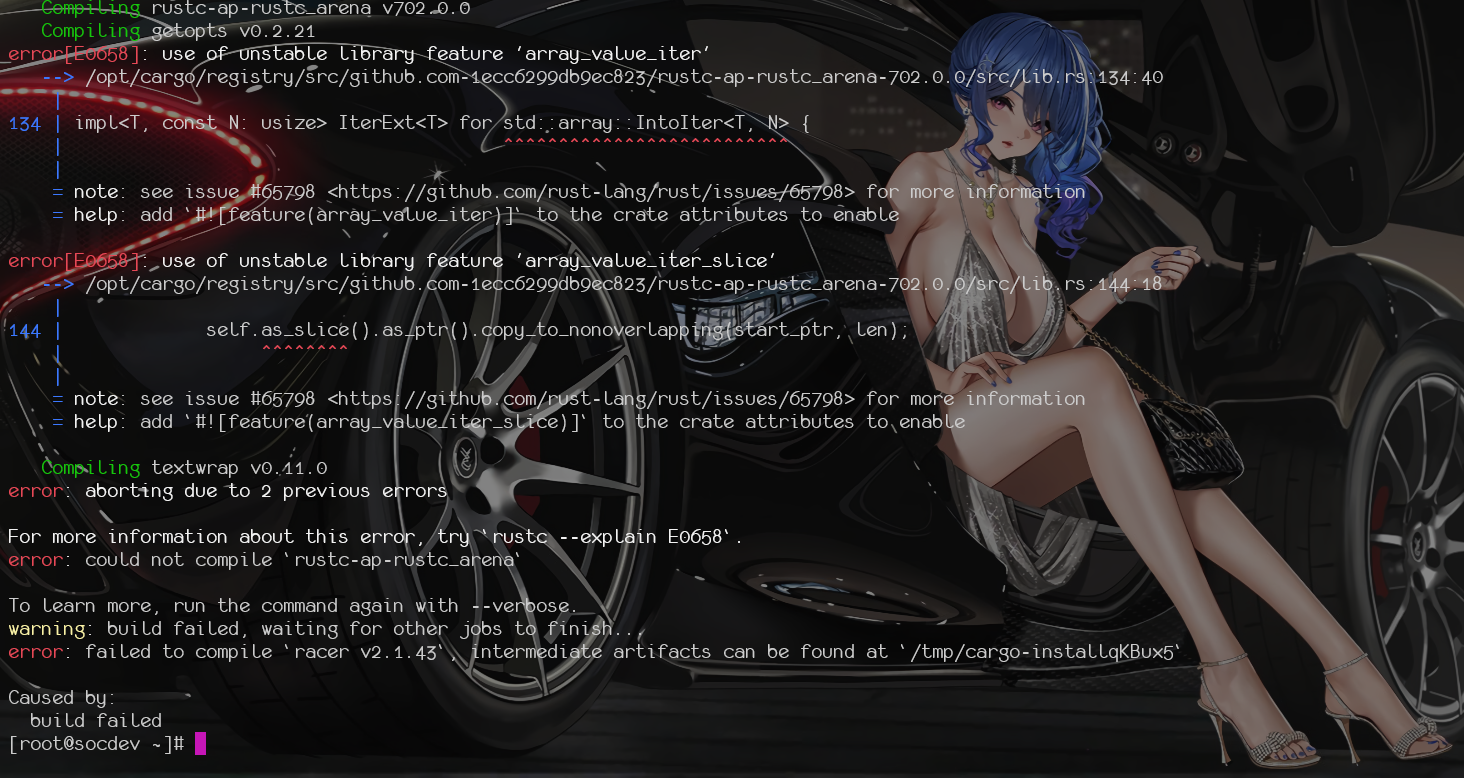
\includegraphics[width=\linewidth]{rust_feature_error.png}
  \caption{缺少特性支持编译失败}
  \label{fig:rust_feature_error}
\end{figure}
遇到这种错误,则需要直接修改对应的类库的源代码。以上述错误为例,编译的help表示
\mintinline[breaklines=true,breakanywhere,breaksymbolleft=,breakanywheresymbolpre=,]{bash}{add `#![feature(array_value_iter_slice)]` to the crate attributes to enable},
则我们应当在对应的crate的lib.rs的头部当中,添加内容如下:
\begin{figure}[H]
  \centering
  
\includegraphics[width=\linewidth]{rust_feature_add.png}
  \caption{增加特性支持}
  \label{fig:rust_feature_add}
\end{figure}
